\chapter{ElmerGrid mesh manipulation examples}

ElmerGrid may often be used as a grid manipulation
tool even though the computational mesh would 
originally have been made by some other mesh
generator. There are many basic 
operations, such as scaling or rotation, which do not 
require any special attention. Here we look at some more 
advanced things that may be performed an a mesh. 



\section{Mesh partitioning}

Nowadays the best performance from computers is obtained using
parallel solution techniques. In finite element method this
means that the mesh must be divide into separate domains 
that are solved by single processors. The domains should 
be chosen so that the extra work needed for the communications is
minimized. This procedure is called mesh partitioning. 
ElmerGrid offers two different techniques for this. 
The first one used Metis library and the second one divides the
mesh using simple ordering schemes. 

As an example we choose an L-shaped domain of bilinear elements.
The grid file for creating this one is given below.
\verbatiminput{tool/angle.grd}

The partitioning may be invoked using command line arguments, or
as here using command file. Below is the command file
for using the simple partitioning scheme to partition the
mesh into $2 \times 2$ domains. 
%
\verbatiminput{tool/part.eg}
%
In the start of the command file the user defines the input and 
output formats and filenames. The only additional command is the 
last line that defines how the mesh is partitioned.
Another choice is to use Metis which is invoked with the line
\begin{verbatim}
Metis = 4
\end{verbatim}
The resulting partitionings are shown in Figure~\ref{pic50}. In this case
the partitionings are almost equally good. In very simple
cases the simple geometrical algorithm may give better results
but in general cases Metis should be favored.
%
\begin{figure}
\begin{center}

\includegraphics[width=7cm]{part.png}

\includegraphics[width=7cm]{metis.png}
\end{center}
\caption{A simple mesh partitioned with a simple geometrical scheme and 
Metis library.}
\label{pic50}
\end{figure}


\section{Boundary layer creation}

In nature there are often sharp changes in the physical 
behavior which may be seen in forms of boundary layers.
Particularly in the area of fluid dynamics boundary layers
are often of special interest. 
A physical boundary layer requires
a suitable computational mesh if one 
wants to model the physical phenomena accurately. 
Equally tight mesh is not usually needed elsewhere and thus
an optimal solution is a proper boundary layer mesh.
Ideally the mesh is such that the elements are small only in the 
direction of the gradient. 

ElmerGrid includes a simple 2D capability for creating boundary layer
meshes. There the user may choose the boundary conditions of interest 
and extrude them in the direction of the normal to create a structured 
mesh just on the boundary. The new mesh may also be fitted into the 
size of the original mesh using a simple Jacobian smoother which
tries to maintain the geometrical shape of the mesh. 
Often this is not so easy and therefore the methodology may create
some complications on the corner nodes, for example.

The example case chosen is the same one as for the 
partitioning example except the number of plane elements is reduced to
300 to make the boundary layer more visible.
In the geometry there is only one boundary and therefore 
only one boundary layer is also created. There can however be several
boundary layers at a time. In the intersections of different boundary
layers one should however notice that the number of new elements should be
the same. The resulting mesh is shown in Figure~\ref{pic51}.
%
\verbatiminput{tool/layer.eg}

\begin{figure}
\begin{center}
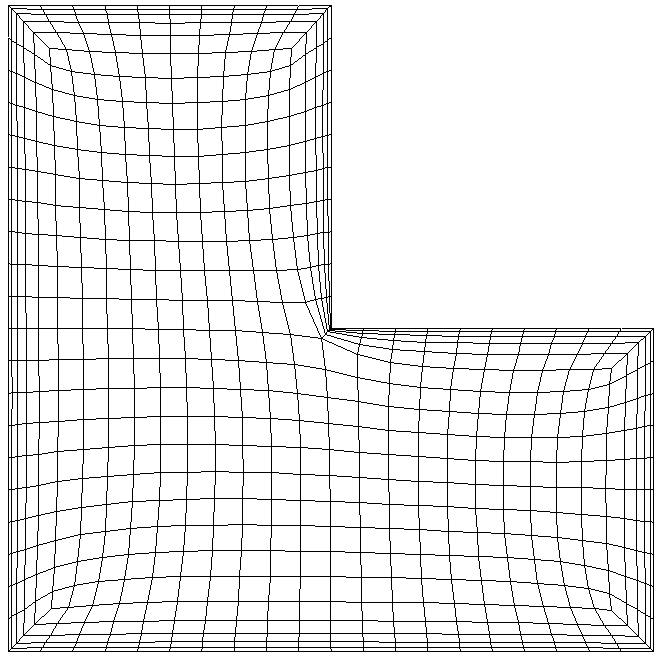
\includegraphics[width=7cm]{layer.png}
\end{center}
\caption{A simple boundary layer created on an angle mesh}
\label{pic51}
\end{figure}

\section{Mesh extrusion}

ElmerGrid enables that any mesh on a plane may be extruded in the 
third dimension by given the specifications on how to extrude.
For example the command file below may be used to extrude the mesh 
created in the first example in the third dimension. The result is a unit 
cube with 1000 trilinear elements.
%
\verbatiminput{tool/rect2cube.eg}
%
\begin{figure}[bh]
\begin{center}
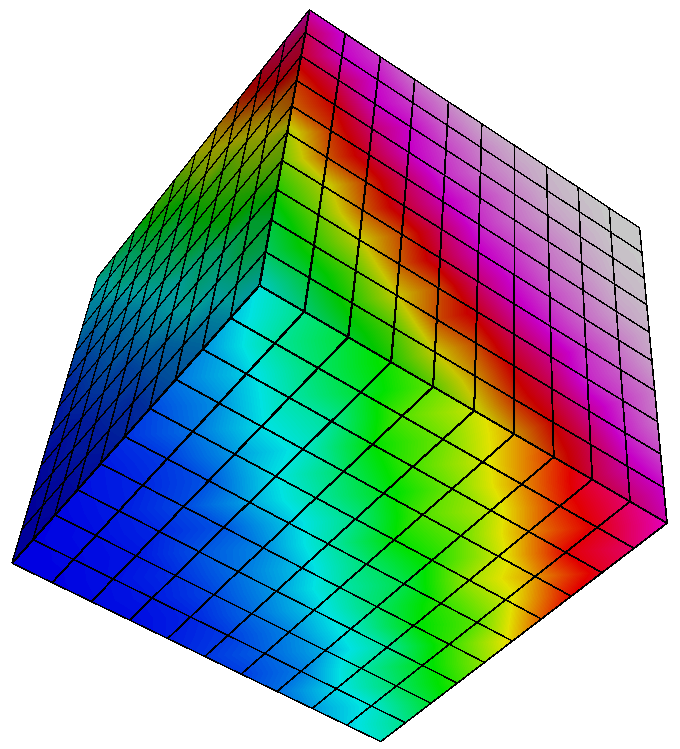
\includegraphics[width=7cm]{cube.png}
\end{center}
\caption{A simple cube created by the extrusion of a unit square}
\label{pic52}
\end{figure}
